\documentclass[oneside]{book}


\usepackage[a4paper,left=0.5in, right=0.5in, top=0.5in, bottom=0.5in]{geometry}
\usepackage{hyperref}
\hypersetup{
    colorlinks=true,    
    urlcolor=cyan,
}
\usepackage{float}

\pagestyle{plain}
\usepackage{titlesec}
\titleformat{\chapter}[hang] 
{\centering \normalfont\Huge\bfseries}{}{1em}{} 

\usepackage{xcolor}

\usepackage{minted}
\usemintedstyle{fruity}

\usepackage{graphicx}
\graphicspath{ {./documentation/Resources/proteusOutput/} }

\newcommand{\pinFormat}[1]{\emph{\textcolor{red}{#1}}}
\newcommand{\regFormat}[1]{\textbf{\textcolor{magenta}{#1}}}

\begin{document}
\tableofcontents

\chapter{Basic Programs}

\section{BasicLedBlink}
\subsection{Circuit}
\begin{figure}[H]
    \centering
    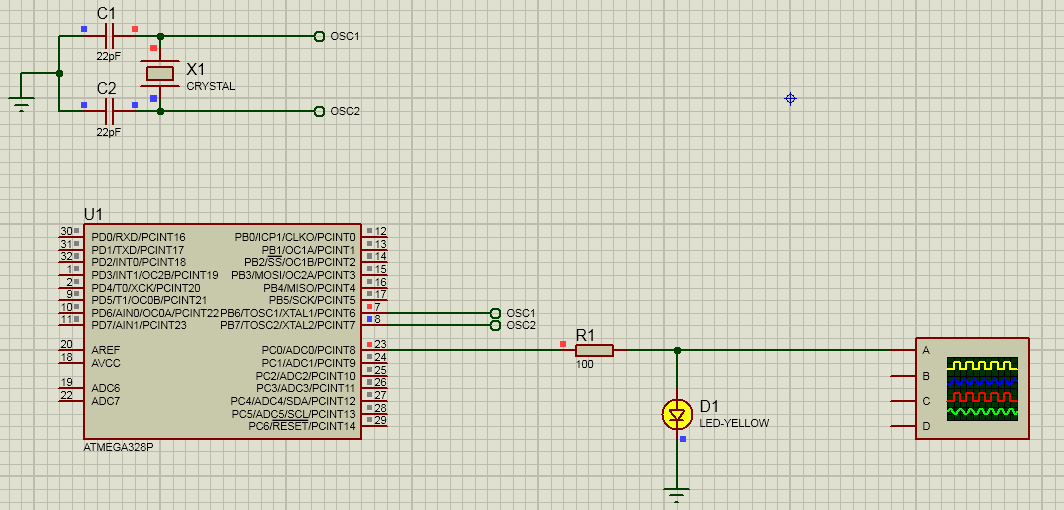
\includegraphics[height=0.2\textheight]{basicLedBlink.png}
\end{figure}
\subsection{Code}
\inputminted[bgcolor=black]{c}{./programFiles/basicLedBlink.c}
\subsection{Output}
\quad The Output can be seen @ \pinFormat{PC0}.


\section{InterruptsExternal}
\subsection{Circuit}
\begin{figure}[H]
    \centering
    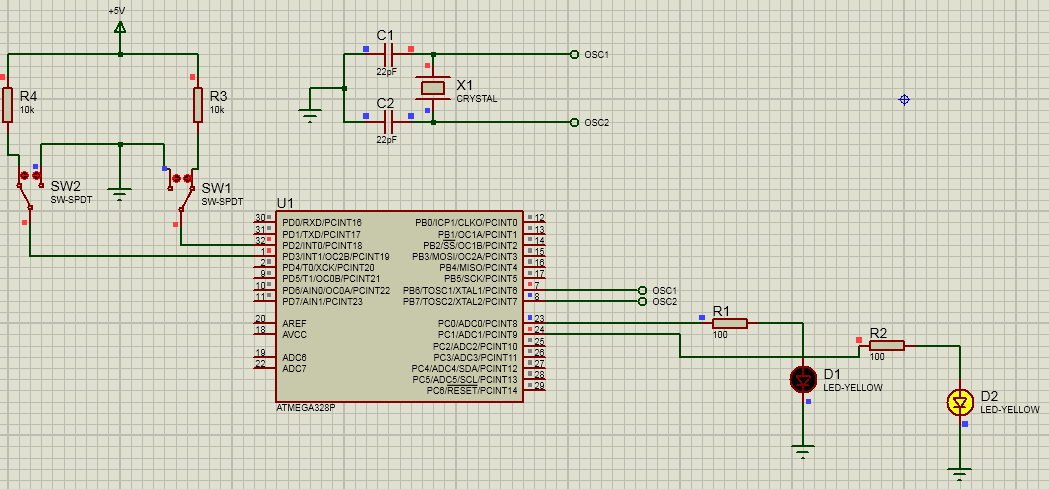
\includegraphics[height=0.2\textheight]{InterruptsExternal.png}
\end{figure}
\subsection{Code}
\inputminted[breaklines,bgcolor=black]{c}{./programFiles/InterruptsExternal.c}
\subsection{Output}
\quad The Output can be seen @ \pinFormat{PC0} and \pinFormat{PC1} when falling edge @ \pinFormat{INT0} and rising edge @ \pinFormat{INT1} occurs.


\section{InterruptsPinChange}
\subsection{Circuit}
\begin{figure}[H]
    \centering
    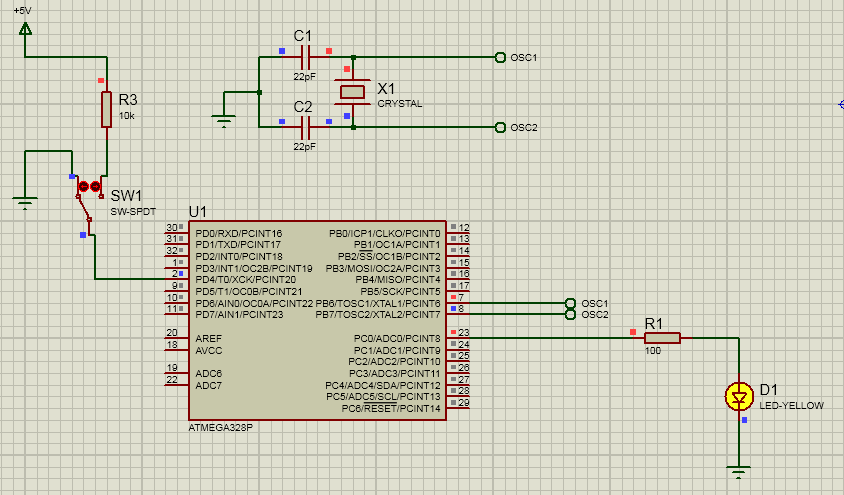
\includegraphics[height=0.2\textheight]{InterruptsPinChange.png}
\end{figure}
\subsection{Code}
\inputminted[breaklines,bgcolor=black]{c}{./programFiles/InterruptsPinChange.c}
\subsection{Output}
\quad The Output can be seen @ \pinFormat{PC0} when pin change @ \pinFormat{PCINT20} occurs.


\section{TimerCounter0\_NormalMode}
\subsection{Circuit}
\begin{figure}[H]
    \centering
    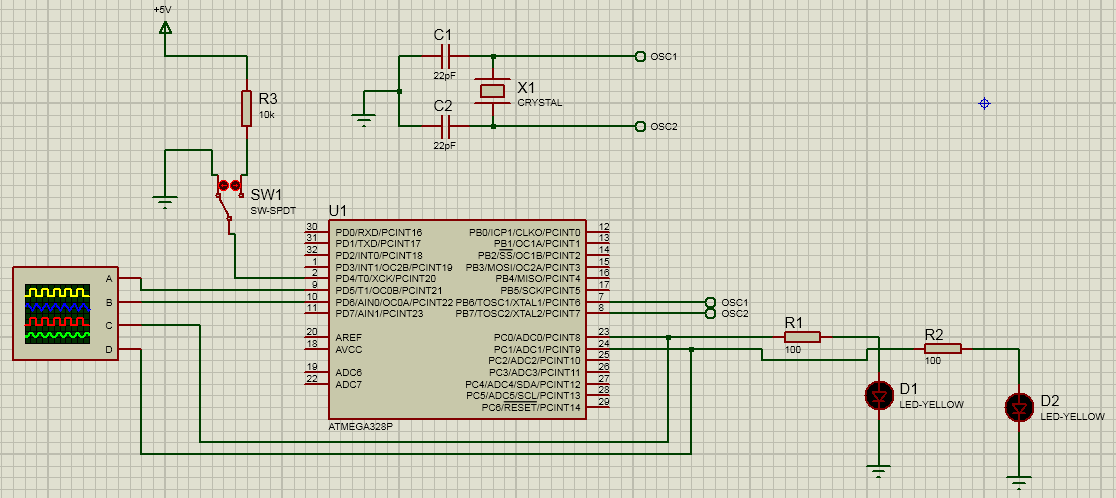
\includegraphics[height=0.2\textheight]{TimerCounter0_NormalMode.png}
\end{figure}
\subsection{Code}

\inputminted[breaklines, bgcolor=black]{c}{./programFiles/TimerCounter0_NormalMode.c}

\subsection{Output}
\subsubsection{Timer0\_asTimer}
\begin{itemize}
    \item The output can be seen @ \pinFormat{OC0A} and \pinFormat{OC0B} pins with a on time of 128$\mu$s and off time of 128$\mu$s ($\frac{0xFF * 8}{16000000} = 127.5\mu s$).
    \item Also, \pinFormat{PC1} toglles for the overflow Timer0.
\end{itemize}
\subsubsection{Timer0\_asCounter}
\begin{itemize}
    \item The output can be seen @ Watch Window and see the \regFormat{TCNT0} register when pulsed @ \pinFormat{T0} pin.
\end{itemize}
\subsubsection{Timer0\_asDelay}
\begin{itemize}
    \item The output can be seen \pinFormat{PC0} pin.
\end{itemize}


\section{TimerCounter0\_CTC}
\subsection{Circuit}
\begin{figure}[H]
    \centering
    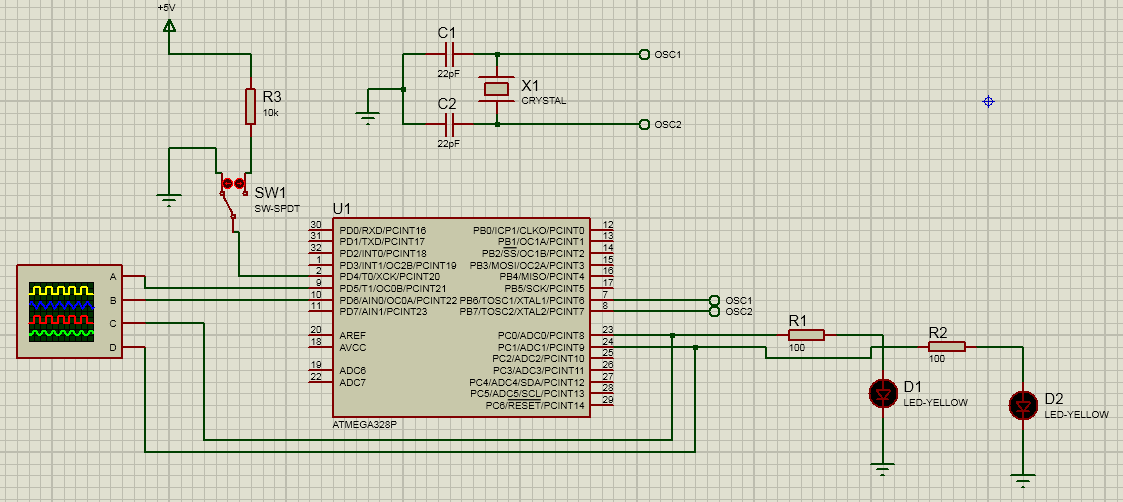
\includegraphics[height=0.2\textheight]{TimerCounter0_CTC.png}
\end{figure}
\subsection{Code}
\inputminted[breaklines, bgcolor=black]{c}{./programFiles/TimerCounter0_CTC.c}
\subsection{Output}
\subsubsection{Timer0\_asTimer}
\begin{itemize}
    \item The output can be seen @ \pinFormat{OC0A} and \pinFormat{OC0B} pins with a on time of 25.5$\mu$s and off time of 25.5$\mu$s ($\frac{(0x32+1) * 8}{16000000} = 25.5\mu s$).
    \item Also, \pinFormat{PC1} toglles for the \regFormat{TCNT0} matches \regFormat{OCR0A}.
\end{itemize}
\subsubsection{Timer0\_asCounter}
\begin{itemize}
    \item The output can be seen @ Watch Window and see the \regFormat{TCNT0} register when pulsed @ \pinFormat{T0} pin.
    \item Also, the \pinFormat{PC1} pin toggles for every 10 changes at \pinFormat{T0} pin.
\end{itemize}
\subsubsection{Timer0\_asDelayIn\_ms}
\begin{itemize}
    \item The output can be seen \pinFormat{PC0} pin.
\end{itemize}


\section{TimerCounter0\_FastPWM}
\subsection{Circuit}
\begin{figure}[H]
    \centering
    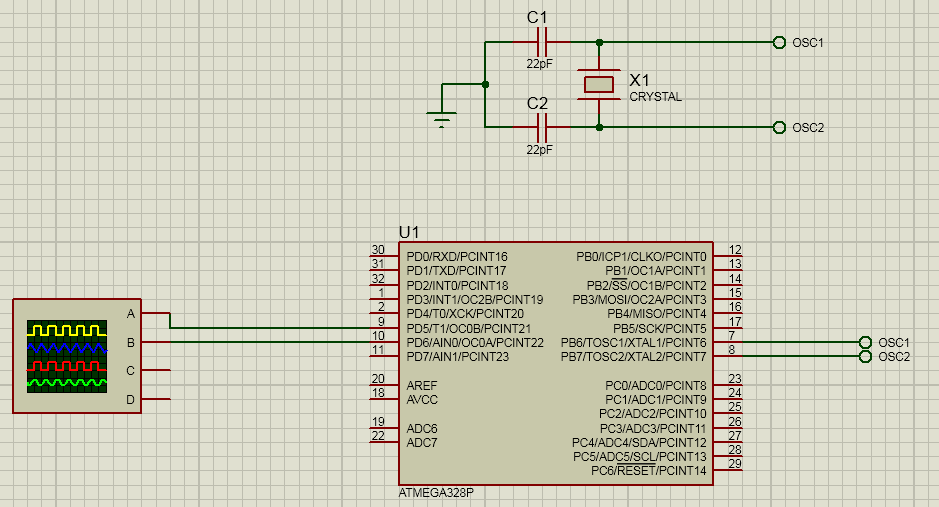
\includegraphics[height=0.2\textheight]{TimerCounter0_FastPWM.png}
\end{figure}
\subsection{Code}
\inputminted[breaklines, bgcolor=black]{c}{./programFiles/TimerCounter0_FastPWM.c}
\subsection{Output}
\subsubsection{Timer0\_NonInverting\_TOP\_at\_MAX}
\begin{itemize}
    \item The output can be seen @ \pinFormat{OC0A} with a frequency of 62.74 kHz($\frac{0xFF * 1}{16000000} = 15.9\mu s$) and duty cycle of 10\% ($\frac{10}{100} * 0xFF = 0x19$).
    \item The output can be seen @ \pinFormat{OC0B} with a frequency of 62.74 kHz($\frac{0xFF * 1}{16000000} = 15.9\mu s$) and duty cycle of 75\% ($\frac{75}{100} = 0xC0$).
\end{itemize}
\subsubsection{Timer0\_Inverting\_TOP\_at\_MAX}
\begin{itemize}
    \item The output can be seen @ \pinFormat{OC0A} with a frequency of 62.74 kHz($\frac{0xFF * 1}{16000000} = 15.9\mu s$) and duty cycle of (100 - 10)\% ($\frac{10}{100} * 0xFF = 0x19$).
    \item The output can be seen @ \pinFormat{OC0B} with a frequency of 62.74 kHz($\frac{0xFF * 1}{16000000} = 15.9\mu s$) and duty cycle of (100 - 75)\% ($\frac{75}{100} = 0xC0$).
\end{itemize}
\subsubsection{Timer0\_NonInverting\_TOP\_at\_OCR0A}
\begin{itemize}
    \item The output can be seen @ \pinFormat{OC0B} with a frequency of 142.857 kHz($\frac{0x70 * 1}{16000000} = 7\mu s$) and duty cycle of 85\% ($\frac{85}{100} = 0x60$).
\end{itemize}
\subsubsection{Timer0\_Inverting\_TOP\_at\_OCR0A}
\begin{itemize}
    \item The output can be seen @ \pinFormat{OC0B} with a frequency of 142.857 kHz($\frac{0x70 * 1}{16000000} = 7\mu s$) and duty cycle of (100 - 85)\% ($\frac{85}{100} = 0x60$).
\end{itemize}
\subsubsection{Timer0\_OC0A\_Square}
\begin{itemize}
    \item The output can be seen @ \pinFormat{OC0A} with a frequency of 142.857 kHz($\frac{0x70 * 1}{16000000} = 7\mu s$).
\end{itemize}
\subsubsection{PWMGeneration}
\begin{itemize}
    \item The output can be seen @ \pinFormat{OC0B}.
\end{itemize}

\section{TimerCounter0\_PhaseCorrectedPWM}
\subsection{Circuit}
\begin{figure}[H]
    \centering
    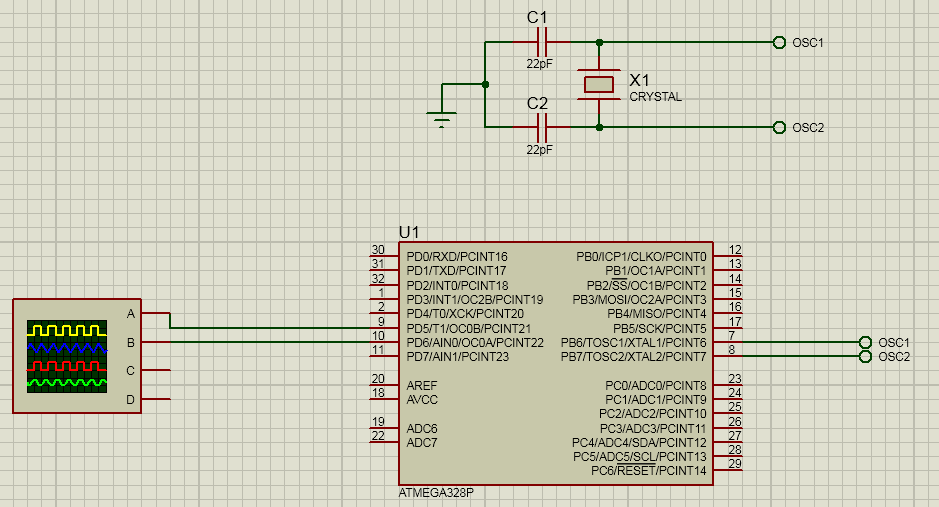
\includegraphics[height=0.2\textheight]{TimerCounter0_PhaseCorrectedPWM.png}
\end{figure}
\subsection{Code}
\inputminted[breaklines, bgcolor=black]{c}{./programFiles/TimerCounter0_PhaseCorrectedPWM.c}
\subsection{Output}
\subsubsection{Timer0\_NonInverting\_TOP\_at\_MAX}
\begin{itemize}
    \item The output can be seen @ \pinFormat{OC0A} with a frequency of 31.372 kHz($\frac{510 * 1}{16000000} = 31.8\mu s$) and duty cycle of 10\% ($\frac{10}{100} * 0xFF = 0x19$).
    \item The output can be seen @ \pinFormat{OC0B} with a frequency of 31.372 kHz($\frac{510 * 1}{16000000} = 31.8\mu s$) and duty cycle of 75\% ($\frac{75}{100} * 0xFF = 0xC0$).
\end{itemize}
\subsubsection{Timer0\_Inverting\_TOP\_at\_MAX}
\begin{itemize}
    \item The output can be seen @ \pinFormat{OC0A} with a frequency of 31.372 kHz($\frac{510 * 1}{16000000} = 31.8\mu s$) and duty cycle of (100 - 10)\% ($\frac{10}{100} * 0xFF = 0x19$).
    \item The output can be seen @ \pinFormat{OC0B} with a frequency of 31.372 kHz($\frac{510 * 1}{16000000} = 31.8\mu s$)and duty cycle of (100 - 75)\% ($\frac{75}{100} * 0xFF = 0xC0$).
\end{itemize}
\subsubsection{Timer0\_NonInverting\_TOP\_at\_OCR0A}
\begin{itemize}
    \item The output can be seen @ \pinFormat{OC0B} with a frequency of 71.42 kHz($\frac{(2*0x70) * 1}{16000000} = 14\mu s$) and duty cycle of 85\% ($\frac{85}{100} * 0x70 = 0x60$).
\end{itemize}
\subsubsection{Timer0\_Inverting\_TOP\_at\_OCR0A}
\begin{itemize}
    \item The output can be seen @ \pinFormat{OC0B} with a frequency of 71.42 kHz($\frac{(2*0x70) * 1}{16000000} = 14\mu s$) and duty cycle of (100 - 85)\% ($\frac{85}{100} * 0x70 = 0x60$).
\end{itemize}
\subsubsection{Timer0\_OC0A\_Square}
\begin{itemize}
    \item The output can be seen @ \pinFormat{OC0A} with a frequency of 71.42 kHz($\frac{(2*0x70) * 1}{16000000} = 14\mu s$).
\end{itemize}
\subsubsection{PWMGeneration}
\begin{itemize}
    \item The output can be seen @ \pinFormat{OC0B}.
\end{itemize}





\section{TimerCounter1\_NormalMode}
\subsection{Circuit}
\begin{figure}[H]
    \centering
    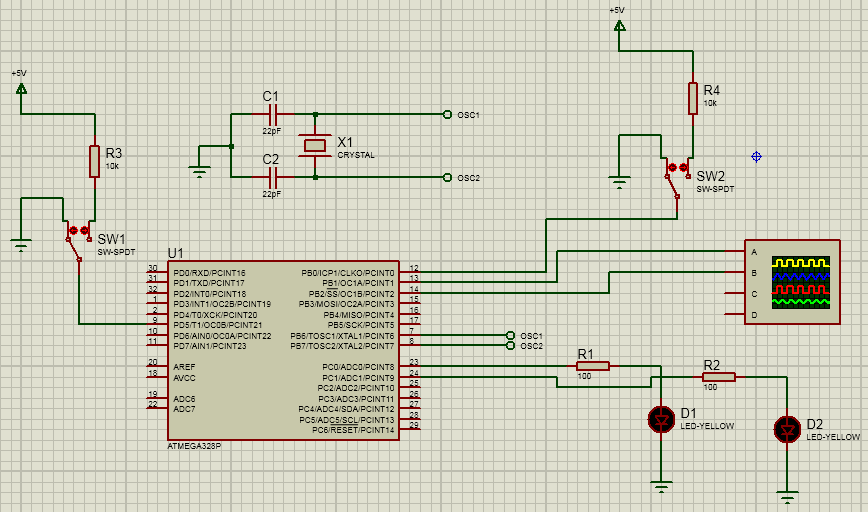
\includegraphics[height=0.2\textheight]{TimerCounter1_NormalMode.png}
\end{figure}
\subsection{Code}
\inputminted[breaklines, bgcolor=black]{c}{./programFiles/TimerCounter1_NormalMode.c}
\subsection{Output}
\subsubsection{Timer1\_asTimer}
\begin{itemize}
    \item The output can be seen @ \pinFormat{OC1A} and \pinFormat{OC1B} pins with a on time of 4.096 ms and off time of 4.096 ms ($\frac{0xFFFF * 1}{16000000} = 4.096 ms$).
    \item Also, \pinFormat{PC1} toggles for the overflow Timer1.
\end{itemize}
\subsubsection{Timer1\_asCounter}
\begin{itemize}
    \item The output can be seen @ Watch Window and see the \regFormat{TCNT1} register when pulsed @ \pinFormat{T1} pin.
\end{itemize}
\subsubsection{Timer1\_asDelay}
\begin{itemize}
    \item The output can be seen \pinFormat{PC0} pin.
\end{itemize}
\subsubsection{Timer1\_asInputCapture}
\begin{itemize}
    \item The output can be seen @ Watch Window and see the \regFormat{ICR1} register when pulsed @ \pinFormat{ICP1} pin.
\end{itemize}

\section{TimerCounter1\_CTC}
\subsection{Circuit}
\begin{figure}[H]
    \centering
    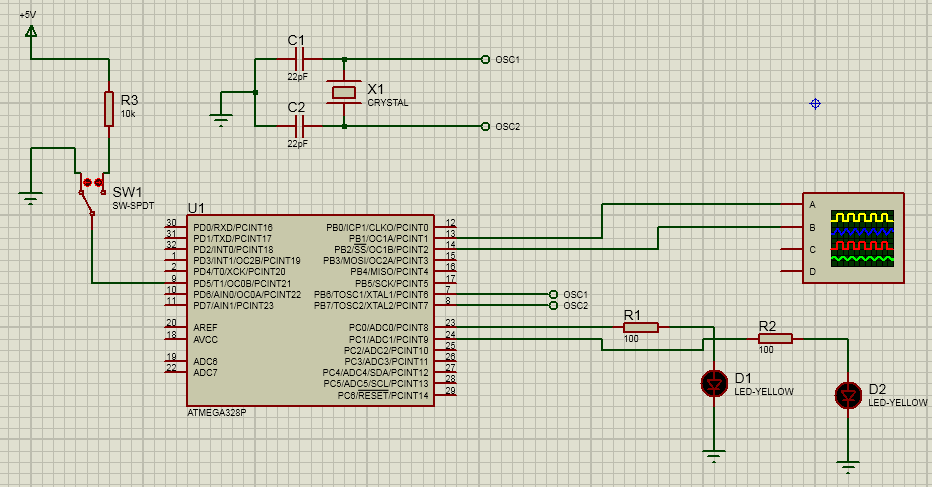
\includegraphics[height=0.2\textheight]{TimerCounter1_CTC.png}
\end{figure}
\subsection{Code}
\inputminted[breaklines, bgcolor=black]{c}{./programFiles/TimerCounter1_CTC.c}
\subsection{Output}
\subsubsection{Timer1\_asTimer}
\begin{itemize}
    \item The output can be seen @ \pinFormat{OC1A} and \pinFormat{OC1B} pins with a on time of 1.15ms and off time of 1.15 ms ($\frac{(0x4861+1) * 1}{16000000} = 1.15 ms$).
    \item Also, \pinFormat{PC1} toglles for the \regFormat{TCNT1} matches \regFormat{OCR1A}.
\end{itemize}
\subsubsection{Timer1\_asCounter}
\begin{itemize}
    \item The output can be seen @ Watch Window and see the \regFormat{TCNT1} register when pulsed @ \pinFormat{T1} pin.
    \item Also, the \pinFormat{PC1} pin toggles for every 10 changes at \pinFormat{T1} pin.
\end{itemize}
\subsubsection{Timer1\_asDelayIn\_us}
\begin{itemize}
    \item The output can be seen \pinFormat{PC0} pin.
\end{itemize}


\section{TimerCounter1\_FastPWM}
\subsection{Circuit}
\begin{figure}[H]
    \centering
    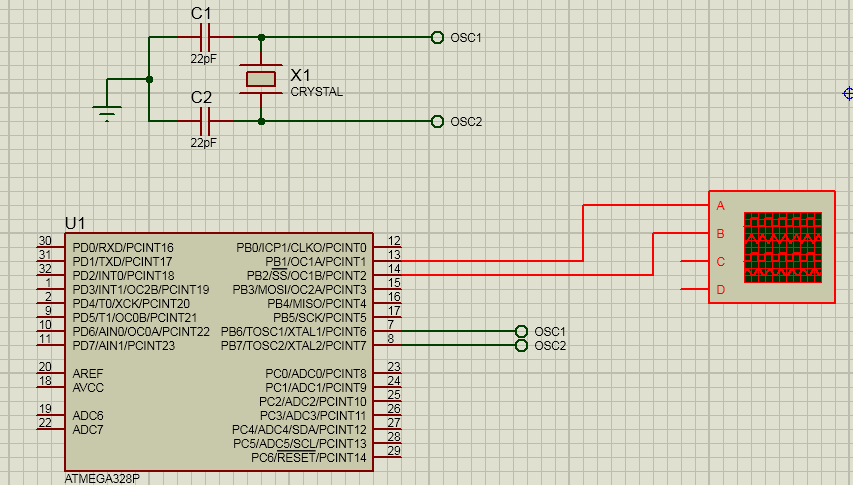
\includegraphics[height=0.2\textheight]{TimerCounter1_FastPWM.png}
\end{figure}
\subsection{Code}
\inputminted[breaklines, bgcolor=black]{c}{./programFiles/TimerCounter1_FastPWM.c}
\subsection{Output}
\subsubsection{Timer1\_NonInverting\_TOP\_at\_MAX}
\begin{itemize}
    \item The output can be seen @ \pinFormat{OC1A} with a frequency of 15.640 kHz($\frac{0x03FF * 1}{16000000} = 64 ms$) and duty cycle of 10\% ($\frac{10}{100} * 0x3FF = 0x66$).
    \item The output can be seen @ \pinFormat{OC1B} with a frequency of 15.640 kHz($\frac{0x03FF * 1}{16000000} = 64 ms$) and duty cycle of 75\% ($\frac{75}{100} * 0x3FF = 0x2FF$).
\end{itemize}
\subsubsection{Timer1\_Inverting\_TOP\_at\_MAX}
\begin{itemize}
    \item The output can be seen @ \pinFormat{OC1A} with a frequency of 15.640 kHz($\frac{0x03FF * 1}{16000000} = 64 ms$) and duty cycle of (100 - 10)\% ($\frac{10}{100} * 0x3FF = 0x66$).
    \item The output can be seen @ \pinFormat{OC1B} with a frequency of 15.640 kHz($\frac{0x03FF * 1}{16000000} = 64 ms$) and duty cycle of (100 - 75)\% ($\frac{75}{100} * 0x3FF = 0x2FF$).
\end{itemize}
\subsubsection{Timer1\_NonInverting\_TOP\_at\_OCR1A}
\begin{itemize}
    \item The output can be seen @ \pinFormat{OC1B} with a frequency of 0.5208 kHz($\frac{0x7869 * 1}{16000000} = 1.92 ms$) and duty cycle of 21\% ($\frac{21}{100} = 0x1A20$).
\end{itemize}
\subsubsection{Timer1\_Inverting\_TOP\_at\_OCR1A}
\begin{itemize}
    \item The output can be seen @ \pinFormat{OC1B} with a frequency of 0.5208 kHz($\frac{0x7869 * 1}{16000000} = 1.92 ms$) and duty cycle of (100 - 21)\% ($\frac{21}{100} = 0x1A20$).
\end{itemize}
\subsubsection{Timer1\_OC1A\_Square}
\begin{itemize}
    \item The output can be seen @ \pinFormat{OC1A} with a frequency of 0.5208 kHz($\frac{0x70 * 1}{16000000} = 1.92 ms$).
\end{itemize}
\subsubsection{PWMGeneration}
\begin{itemize}
    \item The output can be seen @ \pinFormat{OC1B}.
\end{itemize}

\section{TimerCounter1\_PhaseCorrectedPWM}
\subsection{Circuit}
\begin{figure}[H]
    \centering
    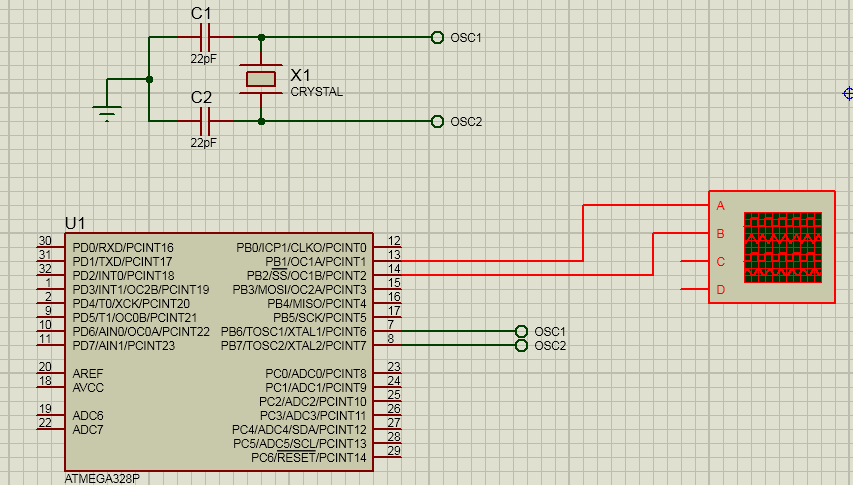
\includegraphics[height=0.2\textheight]{TimerCounter1_PhaseCorrectedPWM.png}
\end{figure}
\subsection{Code}
\inputminted[breaklines, bgcolor=black]{c}{./programFiles/TimerCounter1_PhaseCorrectedPWM.c}
\subsection{Output}\subsubsection{Timer1\_NonInverting\_TOP\_at\_MAX}
\begin{itemize}
    \item The output can be seen @ \pinFormat{OC1A} with a frequency of 7.812 kHz($\frac{(2*0x03FF) * 1}{16000000} = 128 ms$) and duty cycle of 10\% ($\frac{10}{100} * 0x3FF = 0x66$).
    \item The output can be seen @ \pinFormat{OC1B} with a frequency of 7.812 kHz($\frac{(2*0x03FF) * 1}{16000000} = 128 ms$) and duty cycle of 75\% ($\frac{75}{100} * 0x3FF = 0x2FF$).
\end{itemize}
\subsubsection{Timer0\_Inverting\_TOP\_at\_MAX}
\begin{itemize}
    \item The output can be seen @ \pinFormat{OC1A} with a frequency of 7.812 kHz($\frac{(2*0x03FF) * 1}{16000000} = 128 ms$) and duty cycle of (100 - 10)\% ($\frac{10}{100} * 0x3FF = 0x66$).
    \item The output can be seen @ \pinFormat{OC1B} with a frequency of 7.812 kHz($\frac{(2*0x03FF) * 1}{16000000} = 128 ms$) and duty cycle of (100 - 75)\% ($\frac{75}{100} * 0x3FF = 0x2FF$).
\end{itemize}
\subsubsection{Timer1\_NonInverting\_TOP\_at\_OCR1A}
\begin{itemize}
    \item The output can be seen @ \pinFormat{OC1B} with a frequency of 0.2604 kHz($\frac{(2*0x7869) * 1}{16000000} = 3.84 ms$) and duty cycle of 21\% ($\frac{21}{100} = 0x1A20$).
\end{itemize}
\subsubsection{Timer1\_Inverting\_TOP\_at\_OCR1A}
\begin{itemize}
    \item The output can be seen @ \pinFormat{OC1B} with a frequency of 0.2604 kHz($\frac{(2*0x7869) * 1}{16000000} = 3.84 ms$) and duty cycle of (100 - 21)\% ($\frac{21}{100} = 0x1A20$).
\end{itemize}
\subsubsection{Timer1\_OC1A\_Square}
\begin{itemize}
    \item The output can be seen @ \pinFormat{OC1A} with a frequency of 0.2604 kHz($\frac{(2*0x7869) * 1}{16000000} = 3.84 ms$).
\end{itemize}
\subsubsection{PWMGeneration}
\begin{itemize}
    \item The output can be seen @ \pinFormat{OC1B}.
\end{itemize}






\section{TimerCounter2\_NormalMode}
\subsection{Circuit}
\begin{figure}[H]
    \centering
    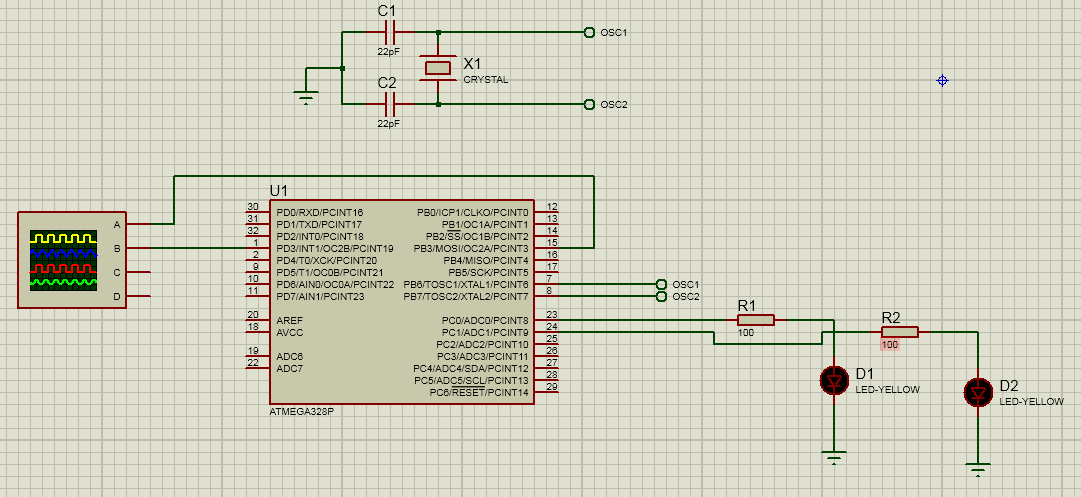
\includegraphics[height=0.2\textheight]{TimerCounter2_NormalMode.png}
\end{figure}
\subsection{Code}
\inputminted[breaklines, bgcolor=black]{c}{./programFiles/TimerCounter2_NormalMode.c}
\subsection{Output}
\subsubsection{Timer2\_asTimer}
\begin{itemize}
    \item The output can be seen @ \pinFormat{OC2A} and \pinFormat{OC2B} pins with a on time of 128$\mu$s and off time of 128$\mu$s ($\frac{0xFF * 8}{16000000} = 127.5\mu s$).
    \item Also, \pinFormat{PC1} toglles for the overflow Timer2.
\end{itemize}
\subsubsection{Timer2\_asDelay}
\begin{itemize}
    \item The output can be seen \pinFormat{PC0} pin.
\end{itemize}


\section{TimerCounter2\_CTC}
\subsection{Circuit}
\begin{figure}[H]
    \centering
    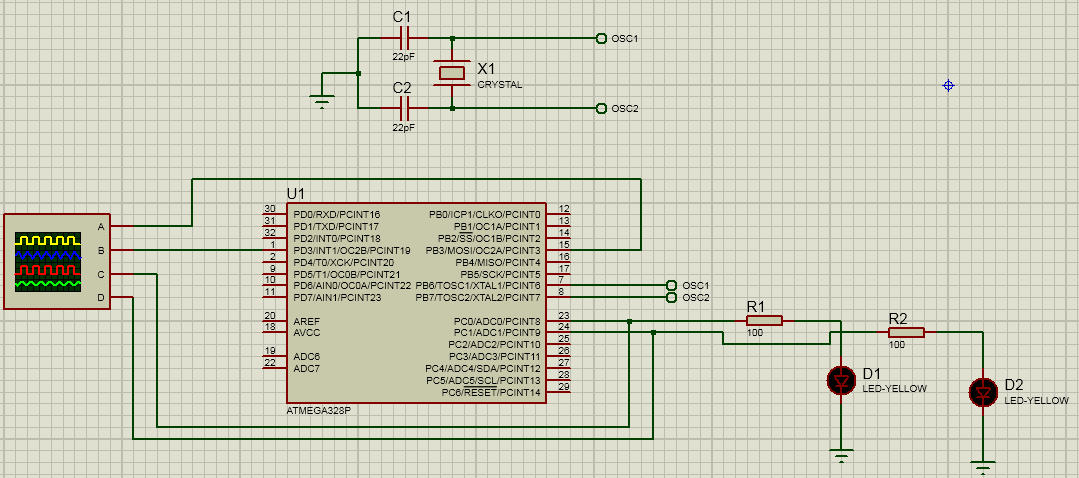
\includegraphics[height=0.2\textheight]{TimerCounter2_CTC.png}
\end{figure}
\subsection{Code}
\inputminted[breaklines, bgcolor=black]{c}{./programFiles/TimerCounter2_CTC.c}
\subsection{Output}
\subsubsection{Timer2\_asTimer}
\begin{itemize}
    \item The output can be seen @ \pinFormat{OC2A} and \pinFormat{OC2B} pins with a on time of 25.5$\mu$s and off time of 25.5$\mu$s ($\frac{(0x32+1) * 8}{16000000} = 25.5\mu s$).
    \item Also, \pinFormat{PC1} toglles for the \regFormat{TCNT2} matches \regFormat{OCR2A}.
\end{itemize}
\subsubsection{Timer2\_asDelayIn\_ms}
\begin{itemize}
    \item The output can be seen \pinFormat{PC0} pin.
\end{itemize}


\section{TimerCounter2\_FastPWM}
\subsection{Circuit}
\begin{figure}[H]
    \centering
    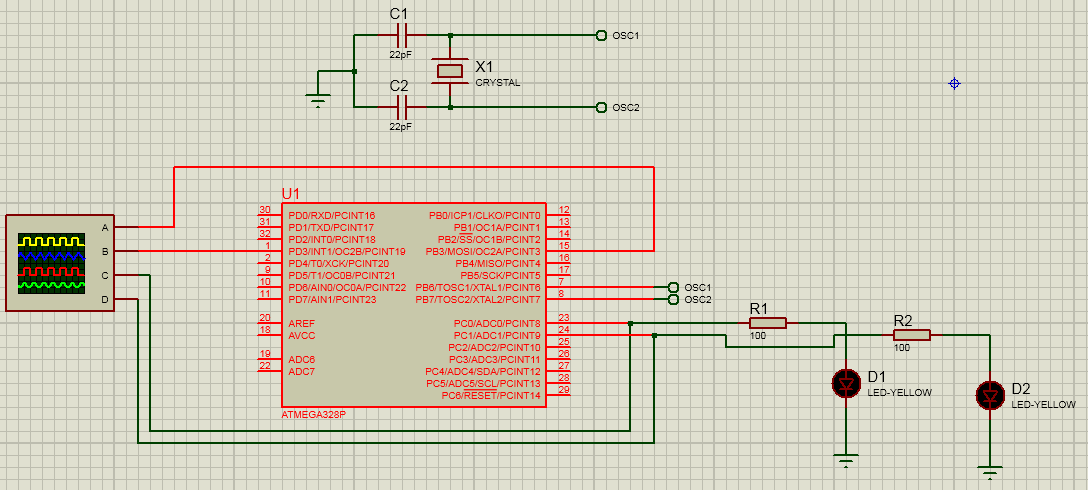
\includegraphics[height=0.2\textheight]{TimerCounter2_FastPWM.png}
\end{figure}
\subsection{Code}
\inputminted[breaklines, bgcolor=black]{c}{./programFiles/TimerCounter2_FastPWM.c}
\subsection{Output}
\subsubsection{Timer2\_NonInverting\_TOP\_at\_MAX}
\begin{itemize}
    \item The output can be seen @ \pinFormat{OC2A} with a frequency of 62.74 kHz($\frac{0xFF * 1}{16000000} = 15.9\mu s$) and duty cycle of 10\% ($\frac{10}{100} * 0xFF = 0x19$).
    \item The output can be seen @ \pinFormat{OC2B} with a frequency of 62.74 kHz($\frac{0xFF * 1}{16000000} = 15.9\mu s$) and duty cycle of 75\% ($\frac{75}{100} = 0xC0$).
\end{itemize}
\subsubsection{Timer2\_Inverting\_TOP\_at\_MAX}
\begin{itemize}
    \item The output can be seen @ \pinFormat{OC2A} with a frequency of 62.74 kHz($\frac{0xFF * 1}{16000000} = 15.9\mu s$) and duty cycle of (100 - 10)\% ($\frac{10}{100} * 0xFF = 0x19$).
    \item The output can be seen @ \pinFormat{OC2B} with a frequency of 62.74 kHz($\frac{0xFF * 1}{16000000} = 15.9\mu s$) and duty cycle of (100 - 75)\% ($\frac{75}{100} = 0xC0$).
\end{itemize}
\subsubsection{Timer2\_NonInverting\_TOP\_at\_OCR2A}
\begin{itemize}
    \item The output can be seen @ \pinFormat{OC2B} with a frequency of 142.857 kHz($\frac{0x70 * 1}{16000000} = 7\mu s$) and duty cycle of 85\% ($\frac{85}{100} = 0x60$).
\end{itemize}
\subsubsection{Timer2\_Inverting\_TOP\_at\_OCR2A}
\begin{itemize}
    \item The output can be seen @ \pinFormat{OC2B} with a frequency of 142.857 kHz($\frac{0x70 * 1}{16000000} = 7\mu s$) and duty cycle of (100 - 85)\% ($\frac{85}{100} = 0x60$).
\end{itemize}
\subsubsection{Timer2\_OC2A\_Square}
\begin{itemize}
    \item The output can be seen @ \pinFormat{OC2A} with a frequency of 142.857 kHz($\frac{0x70 * 1}{16000000} = 7\mu s$).
\end{itemize}
\subsubsection{PWMGeneration}
\begin{itemize}
    \item The output can be seen @ \pinFormat{O20B}.
\end{itemize}

\section{TimerCounter2\_PhaseCorrectedPWM}
\subsection{Circuit}
\begin{figure}[H]
    \centering
    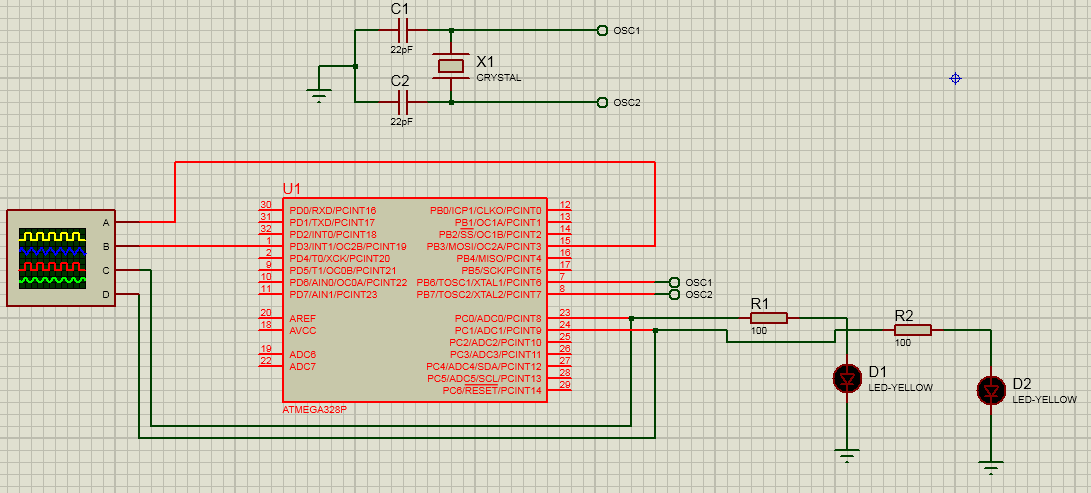
\includegraphics[height=0.2\textheight]{TimerCounter2_PhaseCorrectedPWM.png}
\end{figure}2
\subsection{Code}
\inputminted[breaklines, bgcolor=black]{c}{./programFiles/TimerCounter2_PhaseCorrectedPWM.c}
\subsection{Output}
\subsubsection{Timer2\_NonInverting\_TOP\_at\_MAX}
\begin{itemize}
    \item The output can be seen @ \pinFormat{OC2A} with a frequency of 31.372 kHz($\frac{510 * 1}{16000000} = 31.8\mu s$) and duty cycle of 10\% ($\frac{10}{100} * 0xFF = 0x19$).
    \item The output can be seen @ \pinFormat{OC2B} with a frequency of 31.372 kHz($\frac{510 * 1}{16000000} = 31.8\mu s$) and duty cycle of 75\% ($\frac{75}{100} * 0xFF = 0xC0$).
\end{itemize}
\subsubsection{Timer2\_Inverting\_TOP\_at\_MAX}
\begin{itemize}
    \item The output can be seen @ \pinFormat{OC2A} with a frequency of 31.372 kHz($\frac{510 * 1}{16000000} = 31.8\mu s$) and duty cycle of (100 - 10)\% ($\frac{10}{100} * 0xFF = 0x19$).
    \item The output can be seen @ \pinFormat{OC2B} with a frequency of 31.372 kHz($\frac{510 * 1}{16000000} = 31.8\mu s$)and duty cycle of (100 - 75)\% ($\frac{75}{100} * 0xFF = 0xC0$).
\end{itemize}
\subsubsection{Timer0\_NonInverting\_TOP\_at\_OCR2A}
\begin{itemize}
    \item The output can be seen @ \pinFormat{OC2B} with a frequency of 71.42 kHz($\frac{(2*0x70) * 1}{16000000} = 14\mu s$) and duty cycle of 85\% ($\frac{85}{100} * 0x70 = 0x60$).
\end{itemize}
\subsubsection{Timer2\_Inverting\_TOP\_at\_OCR2A}
\begin{itemize}
    \item The output can be seen @ \pinFormat{OC2B} with a frequency of 71.42 kHz($\frac{(2*0x70) * 1}{16000000} = 14\mu s$) and duty cycle of (100 - 85)\% ($\frac{85}{100} * 0x70 = 0x60$).
\end{itemize}
\subsubsection{Timer2\_OC2A\_Square}
\begin{itemize}
    \item The output can be seen @ \pinFormat{OC2TiA} with a frequency of 71.42 kHz($\frac{(2*0x70) * 1}{16000000} = 14\mu s$).
\end{itemize}
\subsubsection{PWMGeneration}
\begin{itemize}
    \item The output can be seen @ \pinFormat{OC2B}.
\end{itemize}


\section{SPI}
\subsection{Circuit}
\begin{figure}[H]
    \centering
    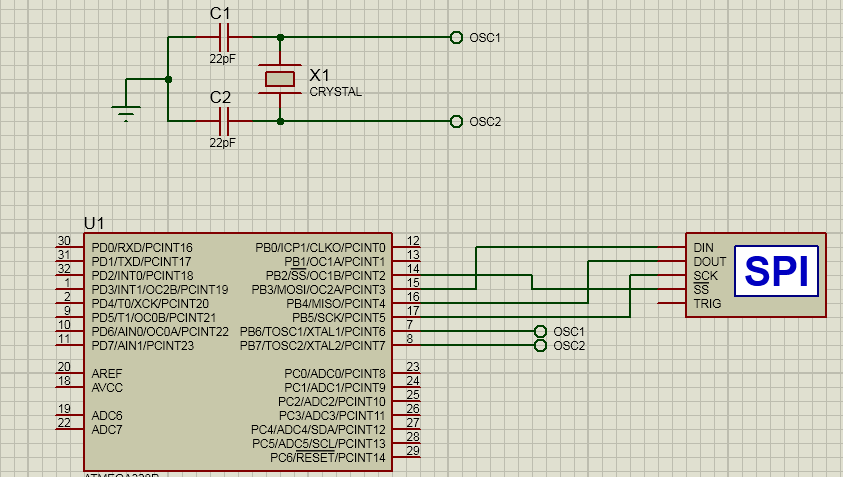
\includegraphics[height=0.2\textheight]{SPI.png}
\end{figure}
\subsection{Code}
\inputminted[bgcolor=black]{c}{./programFiles/SPI.c}
\subsection{Output}
\quad The Output can be seen @ the SPI debugger.


\section{USART0}
\subsection{Circuit}
\begin{figure}[H]
    \centering
    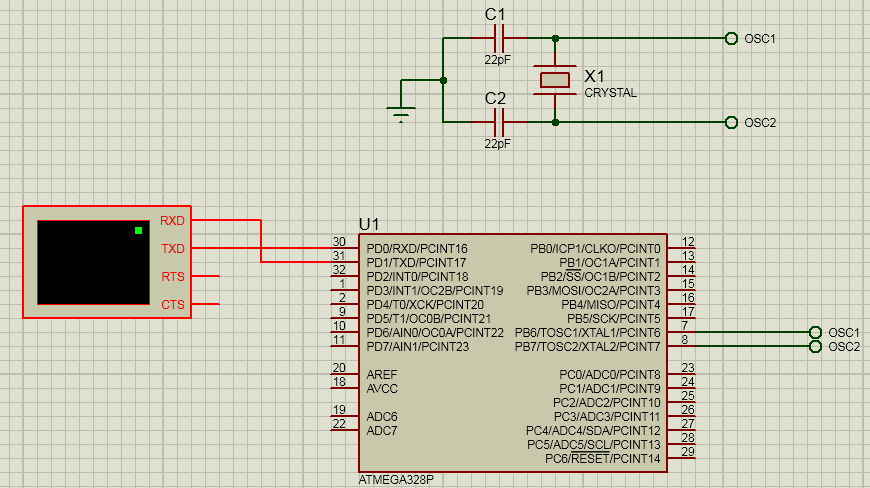
\includegraphics[height=0.2\textheight]{USART0.png}
\end{figure}
\subsection{Code}
\inputminted[bgcolor=black]{c}{./programFiles/USART0.c}
\subsection{Output}
\quad The Output can be seen @ the Virtual Terminal.


\section{TwinWireInterface}
\subsection{Circuit}
\begin{figure}[H]
    \centering
    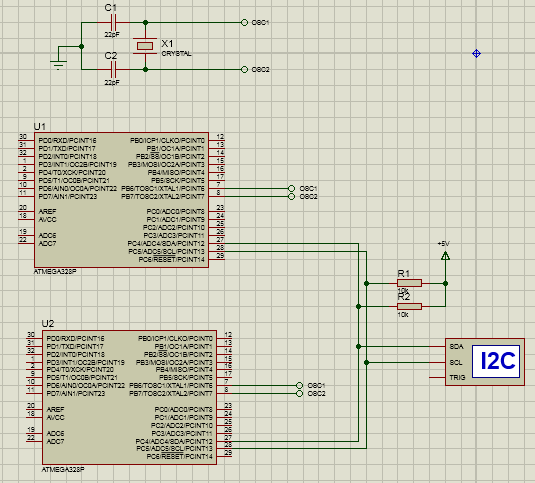
\includegraphics[height=0.2\textheight]{TWI.png}
\end{figure}
\subsection{Code}
\subsubsection{Master Code}
\inputminted[bgcolor=black]{c}{./programFiles/I2C_masterMode.c}
\subsubsection{Slave Code}
\inputminted[bgcolor=black]{c}{./programFiles/I2C_slaveMode.c}
\subsection{Output}
\quad The Output can be seen @ the I2C debugger.


\section{AnalogComparator}
\subsection{Circuit}
\begin{figure}[H]
    \centering
    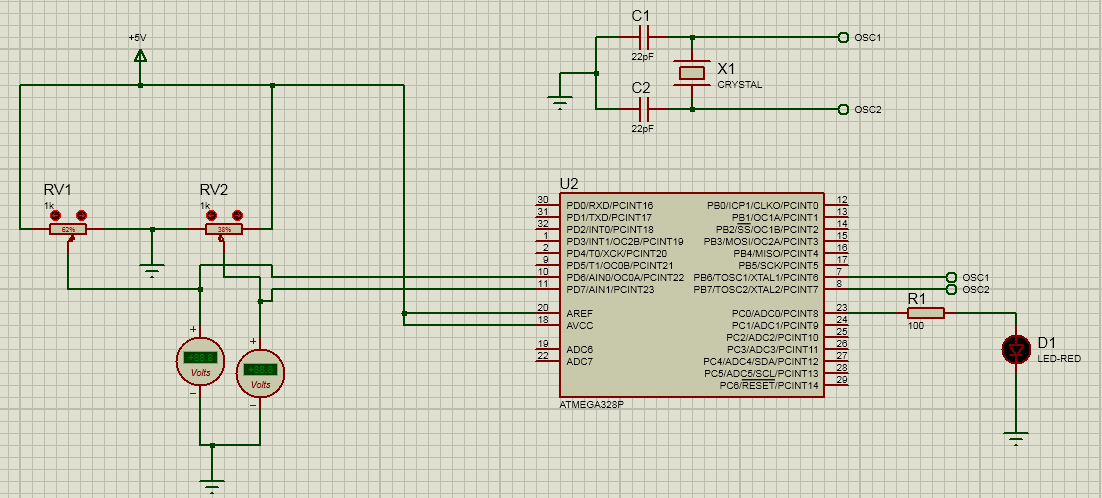
\includegraphics[height=0.2\textheight]{AnalogComparator.png}
\end{figure}
\subsection{Code}
\inputminted[bgcolor=black]{c}{./programFiles/AnalogComparator.c}

\subsection{Output}
\quad The Output can be seen @ \pinFormat{PC0} by changing the voltages.

\section{AnalogToDigital}
\subsection{Circuit}
\begin{figure}[H]
    \centering
    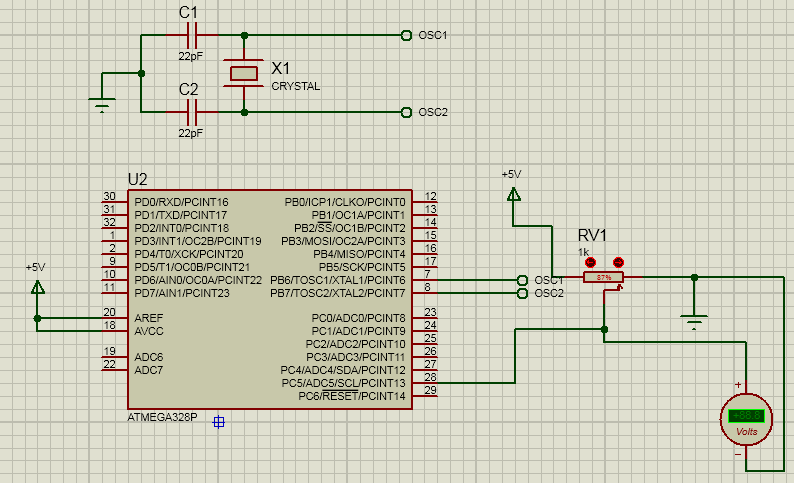
\includegraphics[height=0.2\textheight]{AnalogToDigital.png}
\end{figure}
\subsection{Code}
\inputminted[bgcolor=black]{c}{./programFiles/AnalogToDigital.c}

\subsection{Output}
\quad The Output can be seen @ watch windows by seeing the \regFormat{ADC} register by changing the voltages.


\chapter{Applications}
\section{BasicLCD}
\subsection{Circuit}
\begin{figure}[H]
    \centering
    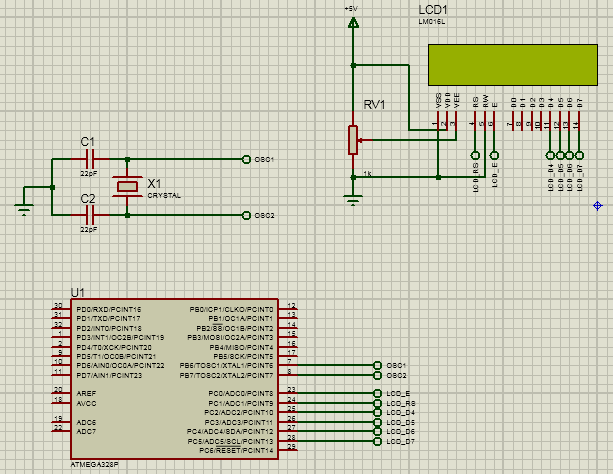
\includegraphics[height=0.2\textheight]{BasicLCD.png}
\end{figure}
\subsection{Code}
\inputminted[bgcolor=black]{c}{./programFiles/BasicLCD.c}

\subsection{Output}
\quad The Output can be seen @ the LCD display.

\section{UARTLCD}
\subsection{Circuit}
\begin{figure}[H]
    \centering
    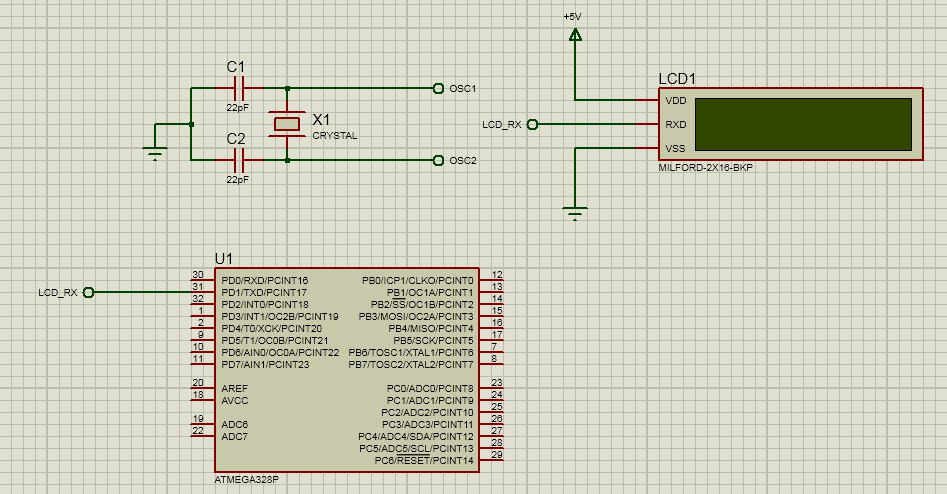
\includegraphics[height=0.2\textheight]{UARTLCD.png}
\end{figure}
\subsection{Code}
\inputminted[bgcolor=black]{c}{./programFiles/UARTLCD.c}

\subsection{Output}
\quad The Output can be seen @ the LCD display.

\section{SPILCD}
\subsection{Circuit}
\begin{figure}[H]
    \centering
    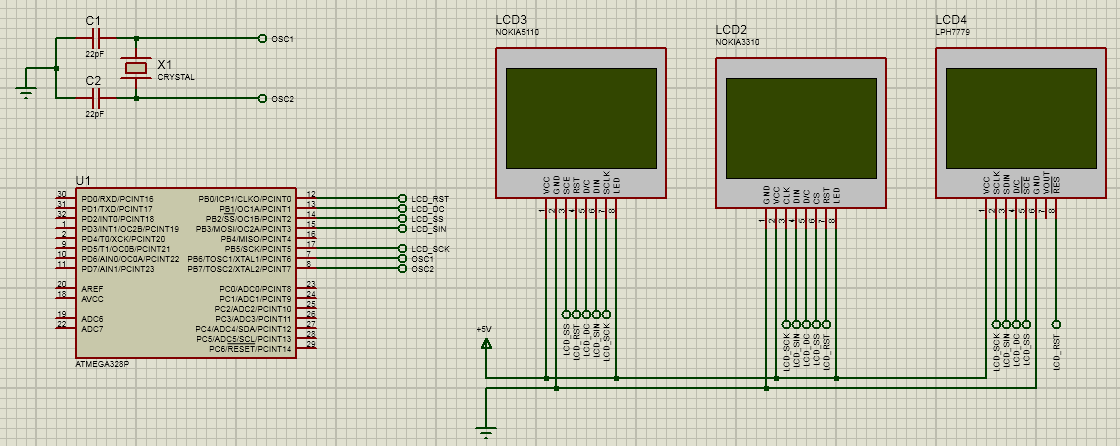
\includegraphics[height=0.2\textheight]{SPILCD.png}
\end{figure}
\subsection{Code}
\inputminted[bgcolor=black]{c}{./programFiles/SPILCD.c}

\subsection{Output}
\quad The Output can be seen @ the LCD display.

\section{I2CLCD}
\subsection{Circuit}
\begin{figure}[H]
    \centering
    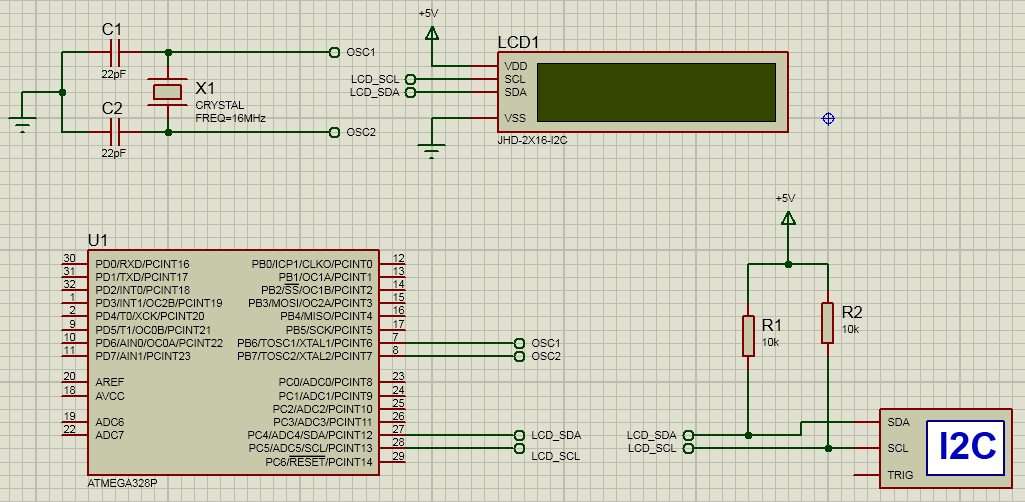
\includegraphics[height=0.2\textheight]{I2CLCD.png}
\end{figure}
\subsection{Code}
\inputminted[bgcolor=black]{c}{./programFiles/I2CLCD.c}

\subsection{Output}
\quad The Output can be seen @ the LCD display.



\section{I2CEEPROM}
\subsection{Circuit}
\begin{figure}[H]
    \centering
    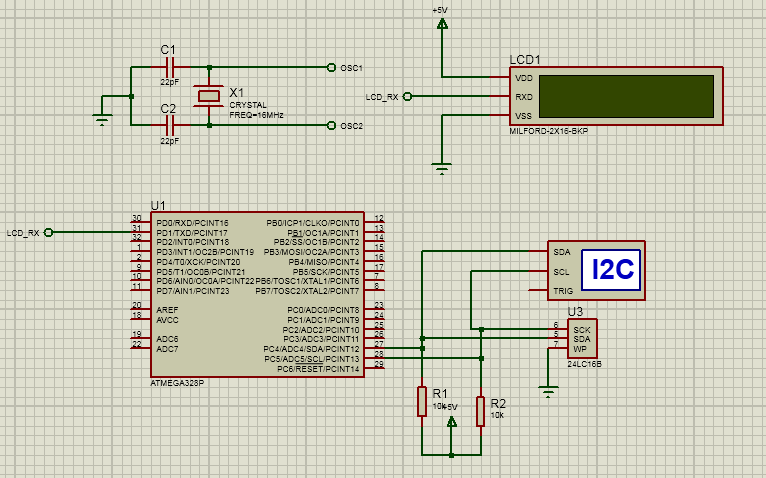
\includegraphics[height=0.2\textheight]{I2CEEPROM.png}
\end{figure}
\subsection{Code}
\inputminted[bgcolor=black]{c}{./programFiles/I2CEEPROM.c}

\subsection{Output}
\quad The Output can be seen @ the LCD display and EEPROM memory.







\chapter{APPENDIX}
\section*{Basic Setup}
\begin{itemize}
    \item The programs are compiled using \emph{\textbf{CompileAndProgram}} script.
    \item The proteus setup is as follows:
    \begin{itemize}
        \item CLKDIV8 - Unprogrammed
        \item CKOUT - Unprogrammed
        \item RSTDISB - Unprogrammed
        \item WDTON - Unprogrammed
        \item BOOTRST - Unprogrammed
        \item CKSEL Fuses - (0110) - External Full-swing Crystall
        \item Boot Loader Size - 00
        \item SUT Fuses - 10
        \item Clock frequency - 160000000
    \end{itemize}
\end{itemize}
\begin{figure}[H]
    \centering
    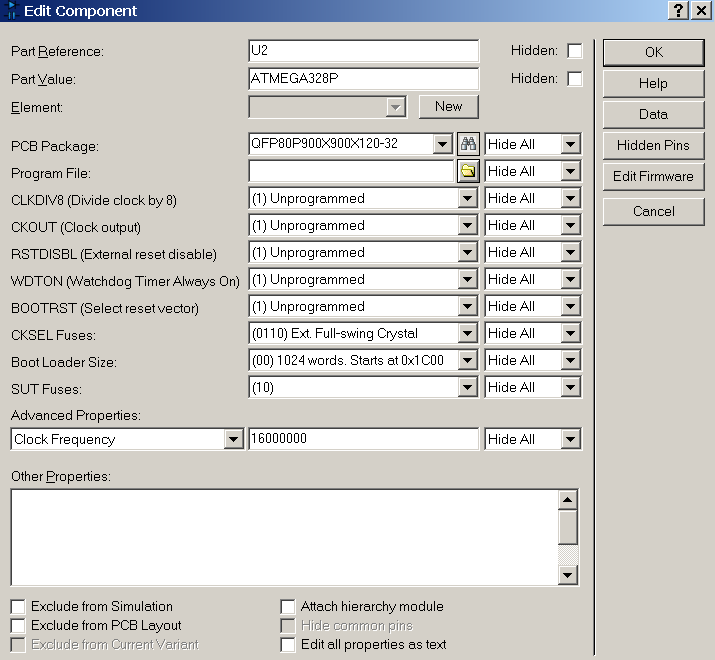
\includegraphics[height=0.75\textwidth]{setup.png}
\end{figure}

\end{document}